\documentclass[11pt]{article}
\usepackage{sectsty}
\usepackage{graphicx}
\graphicspath{{img/}{../img/}{doc/img/}}
\usepackage{listings}
\lstset{language=Matlab}
\usepackage{hyperref}
\usepackage{amsmath}
\usepackage{import}
\usepackage{subfiles}
\usepackage[utf8]{inputenc}
\usepackage[english]{babel}

\usepackage[square, numbers]{natbib}
\bibliographystyle{unsrtnat}
\usepackage[nottoc]{tocbibind}

%\usepackage{biblatex}
%\addbibresource{citations.bib} %usage \cite{test}
% Margins
% 

\topmargin=-0.45in
\evensidemargin=0in
\oddsidemargin=0in
\textwidth=6.5in
\textheight=9.0in
\headsep=0.25in

\title{RNF projekt: Detekce chyby}
\date{\today}
\author{ Artyom Voronin, Martin Havelka, Tomáš Kopčil, Jan Bolcek, Jan Hrůzek}

\begin{document}
\maketitle	

% Optional TOC
\tableofcontents
\pagebreak




\section{Instalace}\label{instalace}}

\begin{itemize}
\tightlist
\item
  Instalace potřebných balíčků:
\end{itemize}

\begin{verbatim}
pip install -r requirements.txt
\end{verbatim}

\begin{itemize}
\item
  Instalace \href{https://pytorch.org/get-started/locally/}{PyTorch}
\end{itemize}

\section{Model a generování dat}\label{model-a-generovuxe1nuxed-dat}}

Jako model byl použit jednoduchý mechanický oscilátor skládající se z
tělesa, pružiny a tlumiče. Parametry tohoto systému jsou tedy hmostnost
\emph{m}, tuhost pružiny \emph{k} a tlumení \emph{b} (podle přiloženého
obrázku \ref{fig:model}).

\begin{figure}[h!]
    \centering
    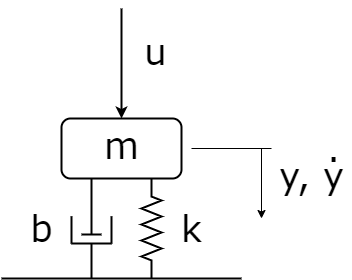
\includegraphics[width=0.4\textwidth]{harmonic_oscillator.png}
    \caption{Harmonic oscillator model}
    \label{fig:model}
\end{figure}

Model je popsán differenciální rovnicí:

\begin{align*}
    m \ddot{y} + b \dot{y} + ky = u(t)
\end{align*}

Oscilátor byl buzen signálem \emph{u(t)} se skokovým průběhem a měrena
byla výchylka a rychlost tělesa.

\hypertarget{generovuxe1nuxed-korektnuxedch-a-chybnuxfdch-dat}{%
\section{Generování korektních a chybných
dat}\label{generovuxe1nuxed-korektnuxedch-a-chybnuxfdch-dat}}

Pro zmíněný model bylo vygenerováno sto různých kombinací parametrů a
pro ně naměřena odezva. Tato data byla označena jako korektní. Jako
chybná byla uvažována situace, kdy se v praxi "utrhne" pružina nebo
tlumič, tedy \emph{k = 0} nebo \emph{b = 0}. Dále také, pokud je poměrný
útlum soustavy větší, nebo roven jedné, tedy soustava je přetlumená a
nedochází ke kmitání.

\hypertarget{statistickuxe9-zpracovuxe1nuxed-dat}{%
\section{Statistické zpracování
dat}\label{statistickuxe9-zpracovuxe1nuxed-dat}}

Detekce chyby probíhala na základě signálu, jeho statistickém zpracování
(signal based fault detection).

Pro každý balík naměřených dat byla zpracována statistická analýza.
Určeny byly následující statistické parametry:

\begin{itemize}
\item
  minimum
\item
  maximum
\item
  aritmetický průměr
\item
  medián
\item
  standardní odchylka
\item
  rozptyl
\item
  RMS
\item
  Fourierova transformace pomocí FFT algoritmu a následně vybrány 3
  nejvíce dominantní frekvence.
\end{itemize}

Tyto parametry byly zabaleny společně s označením (label), zda se jedná
o chybná, nebo korektní data, a následně použita jako dataset pro
neuronovou síť. Pro práci s daty byla využity struktury knihovny
\emph{numpy}, které je následně Pytorch schopen zkonvertovat do svého
formátu.

\hypertarget{dataset}{%
\section{Dataset}\label{dataset}}

Ze statisticky zpracovaných dat byl vytvořen dataset, který odpovídá
vstupům neuronové sítě. Jedná se o tensor,\\
který obsahuje hodnoty features (statistické parametry) a labels
(označení správných a chybných dat, 1/0). Následně byl dataset rozdělen
na trénovací a validační data v poměru 80\% ku 20\%. Takto rozdělený
dataset byl dále použit v neuronové síti.

\hypertarget{neuronovuxe1-suxedux165}{%
\section{Neuronová síť}\label{neuronovuxe1-suxedux165}}

Pro vytvoření neuronové sítě byl použit nástroj PyTorch. Byl vytvořen
model s jednou vstupní, skrytou a výstupní vrstvou.

\hypertarget{velikost-vsrtev}{%
\paragraph{Velikost vsrtev:}\label{velikost-vsrtev}}

\begin{verbatim}
  Vstupní vrstva: 20
  Skrytá vrstva: 16
  Výstupní vrstva: 1
\end{verbatim}

\hypertarget{parametry-suxedtux11b}{%
\paragraph{Parametry sítě:}\label{parametry-suxedtux11b}}

\begin{verbatim}
  Aktivační funkce: sigmoid
  Optimizator: Adam 
  Loss function: MSELoss 
  Learning rate: 0,05 
  Počet epoch: 500 
  Velikost batch: 5
\end{verbatim}

Trénování neuronové sítě tedy probíhalo v závislosti na velikosti batch
a na počtu epoch. Výsledky trénování jsou zobrazeny v následující části.

\hypertarget{vuxfdsledky}{%
\section{Výsledky}\label{vuxfdsledky}}

Následující grafy přestavují chování neuronové sítě při známých
vstupních a neznámých vstupních datech (na kterých nebyla naučena).
Znázorňují postupné ustálení odchylky s narůstajícím počtem epoch
\ref{fig:loss}, \ref{fig:eval}.\\
~\\

\begin{figure}[h!]
    \centering
    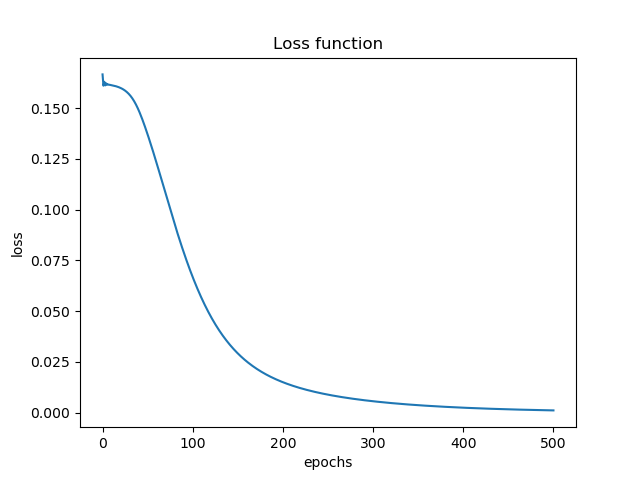
\includegraphics[width=0.8\textwidth]{loss.png}
    \caption{Loss function}
    \label{fig:loss}
\end{figure}

\begin{figure}[h!]
    \centering
    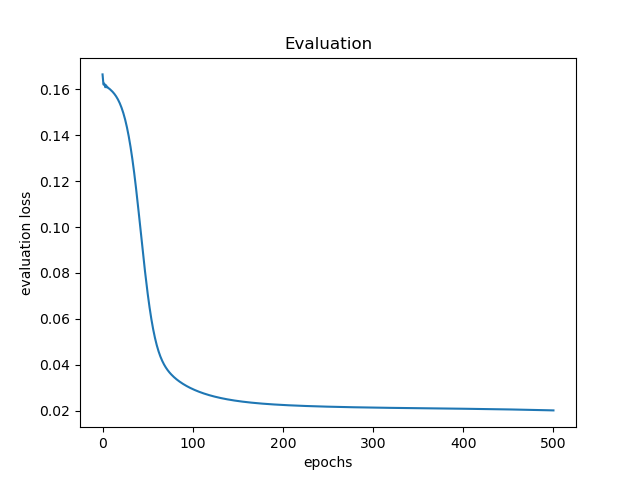
\includegraphics[width=0.8\textwidth]{eval.png}
    \caption{Evaluation}
    \label{fig:eval}
\end{figure}

Při testovacím běhu neuronové sítě byly dosaženy následující výsledky:

\begin{figure}[h!]
    \centering
    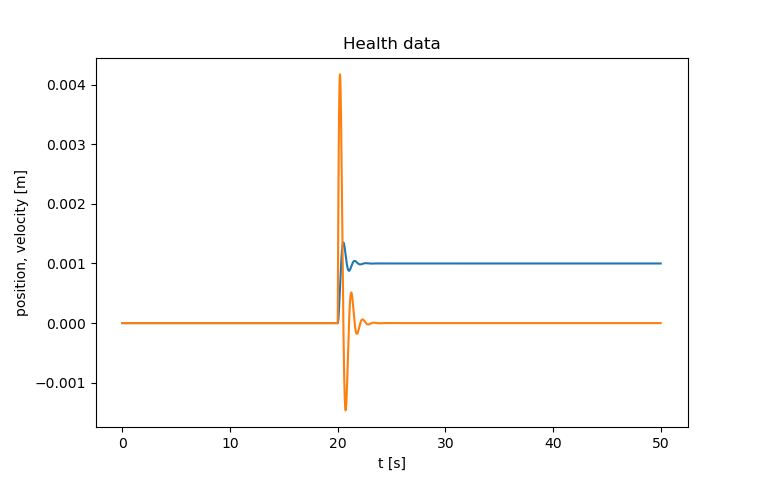
\includegraphics[width=0.8\textwidth]{health.png}
    \caption{Loss function}
    \label{fig:health}
\end{figure}

\begin{figure}[h!]
    \centering
    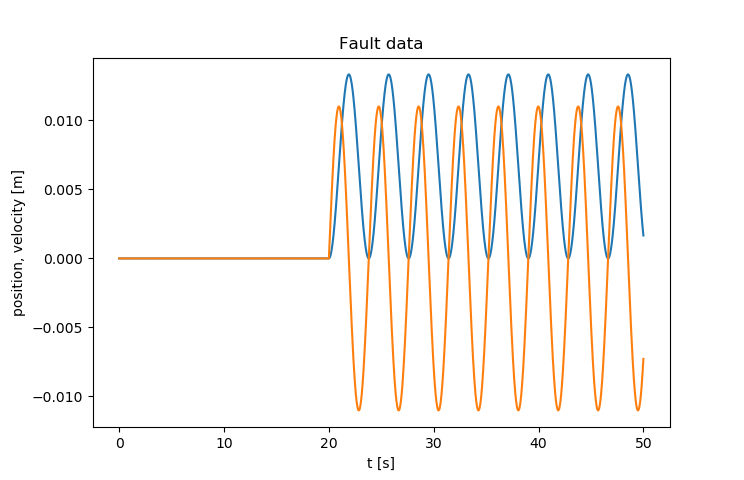
\includegraphics[width=0.8\textwidth]{fault.png}
    \caption{Evaluation}
    \label{fig:fault}
\end{figure}

\begin{verbatim}
[TEST] CASE 1 "Health data" : label=1.0 net_output=0.9970
[TEST] CASE 2 "Fault data " : label=0.0 net_output=0.0000
\end{verbatim}

Na modelu byla vygenerována korektní i chybná data pro verifikaci
funkčnosti neuronové sítě. Tato data jsou zobrazena na následujících
obrázcích. První obrázek \ref{fig:health} zobrazuje výchylku a rychlost tělesa v čase pro
korektní, plně funkční, model. Jak jde vidět, rychlost a výchylka jsou
vůči sobě fázově posunuty a poměrně rychle se ustálí -- jedná se o
odezvu na skok, na který tlumená soustava reaguje postupným ustálením.
\\
Druhý obrázek \ref{fig:fault} zobrazuje situaci pro chybný model, konkrétně případ, kdy
se "utrhnul" tlumič\\
a tlumení soustavy je tedy nulové. V tomto případě proto nedochází k
ustálení a soustava kmitá dále se stejnou amplitudou.

\hypertarget{zuxe1vux11br}{%
\section{Závěr}\label{zuxe1vux11br}}

Pro detekci chyb na základě signálu (signal based fault detection)
pomocí neuronové sítě byl vytvořen model, který byl použit pro
generování dat. Tato vygenerována data ve formě signálů byla následně
označena jako korektní a chybná a byla statisticky zpracována pro
neuronovou síť. Poté proběhlo učení neuronové sitě na základě těchto
statiských dat a labelů.\\
Neuronová síť, která byla vytvořena pomocí nástroje PyTorch, obsahuje 20
neuronů ve vstupní vrstvě, 16 neuronů ve skryté vrstvě a 1 neuron ve
výstupní vrstvě a v rámci její aplikace byla použita sigmoidní aktivační
funkce. Nakonec byl proveden testovací běh neuronové sítě a byla
vygenerována verifikační data pro ověření funkčnosti neuronové sítě.
Ukázalo se, že síť poměrně rychle konverguje ke správnému určení, zda se
jedná o korektní, nebo chybný signál.

\hypertarget{zdroje}{%
\section{Zdroje}\label{zdroje}}

\begin{itemize}
\tightlist
\item
  \href{https://en.wikipedia.org/wiki/Fault_detection_and_isolation}{wiki:
  Fault detection and isolation}
\item
  \href{https://pytorch.org/tutorials/beginner/pytorch_with_examples.html\#pytorch-nn}{PyTorch:
  nn}
\item
  \href{https://www.sciencedirect.com/science/article/pii/S1876610218304831}{A
  machine learning approach to fault detection in district heating
  substations}
\item
  \href{https://www.kaggle.com/c/vsb-power-line-fault-detection/notebooks}{kaggle:
  VSB Power Line Fault Detection}
\item
  \href{https://www.researchgate.net/publication/221412815_Fault_detection_methods_A_literature_survey/}{Fault
  detection methods: A literature survey}
\end{itemize}

\end{document}
